% ----------------------------------------------------------
\chapter{Trabalhos relacionados}
\label{relacionados}

\section{História do Monitoramento da Amazônia por meio de Sensoreamento Remoto}

Devido ao valor da Amazônia e da necessidade em protegê-la, é natural o interesse em se desenvolver tecnologias de monitoramento visando preservar este grande patrimônio natural. A história do sensoriamento remoto na região data desde o ano 1975, quando se foram produzidas as primeiras imagens de satélite Landsat, por meio de um sensor MSS ou sensor multi-espectral.  Estas imagens compuseram o primeiro grande mapeamento do território para se verificar o potencial desta tecnologia no monitoramento de desflorestamento.

A experiência contemplou uma área de 55 milhões de hectares referentes a uma região crítica ligada a grandes projetos agropecuários, revelando que 10\% do território já estava desflorestado. Diante da indignação internacional oriunda deste conhecimento, as autoridades brasileiras instauraram uma Comissão Parlamentar de Inquérito, ou CPI, para investigar o tema \cite{hist_amz}. 

Em contrapartida, as imagens coletadas para este estudo contemplavam apenas uma parte crítica do território, levantando a dúvida sobre o estado do resto do território. Em 1988, teve origem o projeto PRODES Analógico (Projeto de Monitoramento do Desmatamento na Amazônia Legal por Satélite), produzindo métricas desmatamento anuais para todo o território amazônico até 2003.

\begin{figure}[htb]
	\centering
	\begin{minipage}{0.9\linewidth}
		\centering
		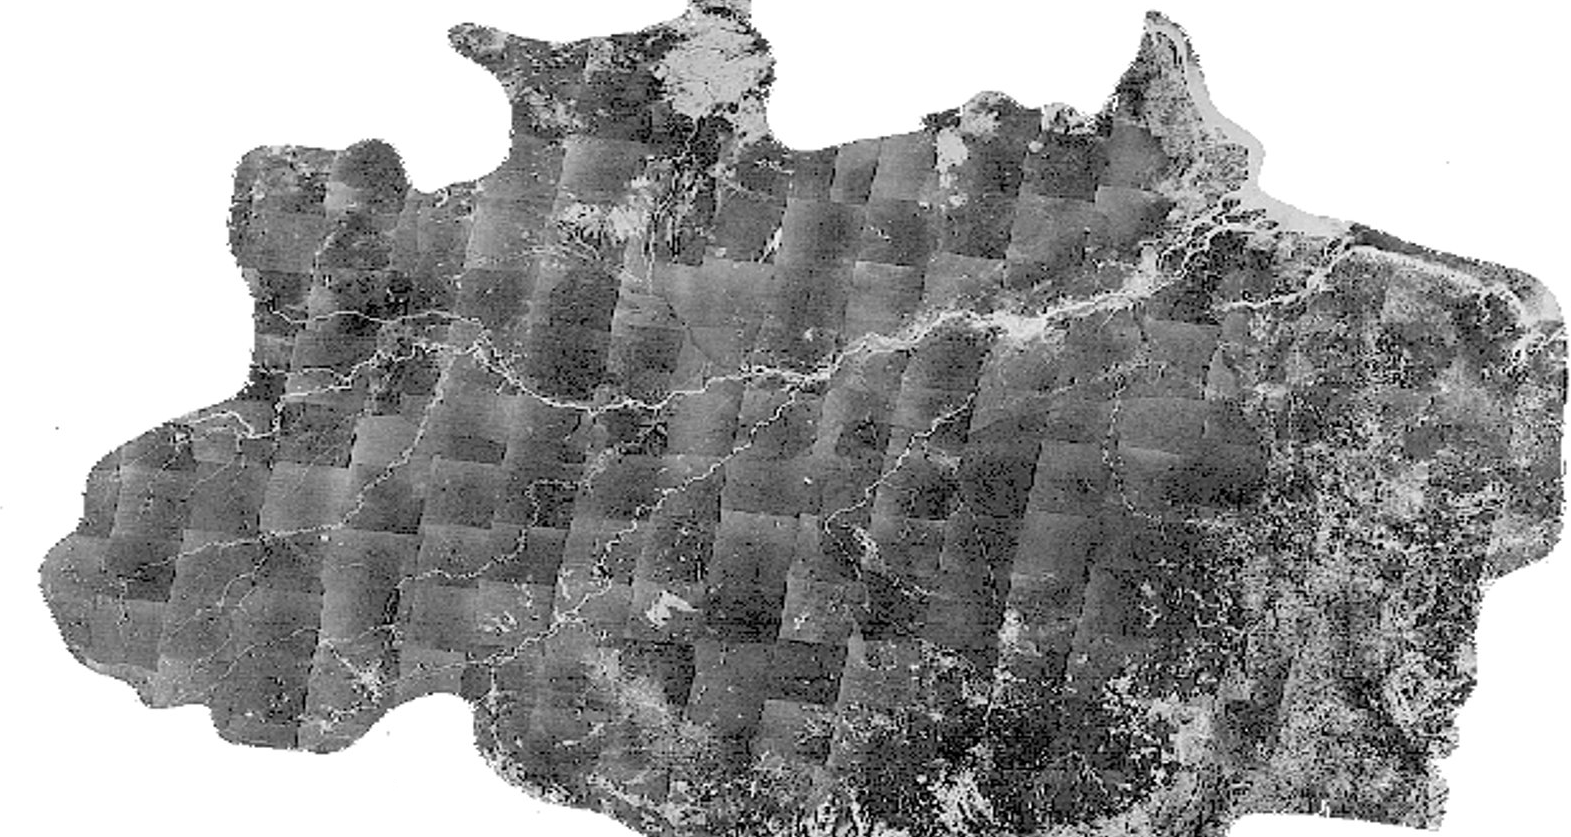
\includegraphics[width=\linewidth]{tg1/figuras/amazon.png}
		\caption{Mosaico com 229 imagens Landsat em escala 1: 250.000 \cite{hist_amz}} \label{fig:amz1988}
	\end{minipage}
\end{figure}

Em sequência, há o nascimento do projeto PANAMAZÔNIA I \cite{panamazonia} em 1992, operando de forma semelhante ao PRODES Analógico. Este novo projeto também faria o monitoramento da Amazônia de forma analógica com imagens do satélite Landsat de resolução 1:250.000, visando aumentar a escala e fazer o monitoramento para toda a América do Sul. 

A próxima etapa desta história se dá em 1997 por meio do PRODES Digital. Este representou um grande avanço tecnológico na forma da criação de um banco de dados digital, porém, foi limitado a operar dentro da complexidade do projeto PRODES Analógico. Por consequência disto, várias melhorias ao sistema de monitoramento e classificação não foram aplicadas.

A partir de 2003 tem-se a origem do projeto DETER (Detecção do Desmatamento em Tempo Real) \cite{deter}. Esta nova empreitada utilizou imagens do sensor MODIS, abordo do satélite Terra. Apesar da baixa resolução das imagens, tinha-se uma alta taxa de amostragem, gerando-se imagens diárias. A partir disto, o sistema fazia a sobreposição destas imagens e polígonos de desmatamento detectados. Caso um polígono de desmatamento fosse sobreposto a uma imagem de vegetação anteriormente intocada, era gerado um alerta de alteração da cobertura vegetal para os órgãos de fiscalização de desmatamento oficiais. Este foi o primeiro sistema de monitoramento em tempo quase real do território amazônico e opera até hoje.

Em 2020 foi lançado pelo \textit{Global Fire Emission Database} o \textit{Amazon Dashboard}, uma ferramenta que rastreia incêndios individuais na região da Amazônia usando uma abordagem para agrupar e classificar as detecções ativas em diferentes tipos de incêndio. O GFED é um banco de dados focado em informações de incêndio obtidos por meio de satélites da NASA como NOAA-20, SUOMI NPP e MODIS \cite{gfed}. No atual estado da arte, o GFED é o único dado a nível mundial com distribuição gratuita na internet que faz referência sobre tipos de fogo. 


Em 2021, o Centro Gestor e Operacional do Sistema de Proteção da Amazônia desenvolve o Painel do Fogo, uma plataforma Web que permite visualizar informações em tempo real sobre incêndios florestais na região da Amazônia com o intuito de subsidiar o acionamento de brigadas ou batalhões durante o combate ao fogo. A novidade se baseia em trabalhar agrupamentos de focos de calor para entender se tal situação é um evento individual de incêndio e queimada, e disponibilizá-los no Mapa Interativo de Incêndios e Queimadas.


%No entanto, a floresta Amazônica compreende um território extremamente extenso com uma mata bastante fechada, implicando em um desafio prático e logístico em sua proteção e monitoramento.

%\todo{tem que readaptar muita coisa}


\section{Outros autores na área de monitoramento ambiental}
% ----------------------------------------------------------


Muitos trabalhos abordam a detecção de incêndios florestais, especialmente usando aprendizado de máquina. Vários sensores podem ser usados, como
como câmeras IP \cite{forest-fire-ip-camera}, sensores sem fio para emissão de monóxido de carbono e temperatura \cite{forest-fire-detection-wireless-sensor} e dados de satélite.

\cite{Abid2021} fornece uma visão geral dos sistemas de detecção e previsão de incêndios florestais com base em algoritmos de aprendizado de máquina.
Os estudos que avaliam os fatores que afetam a ocorrência e o risco de incêndio também são discutidos, juntamente com as principais questões e resultados de cada estudo.

Estudos feitos para o bioma Cerrado mostram grande precisão no mapeamento de cicatrizes de queimaduras. O estudo de Arruda \cite{queimadas_cerrado}  teve como objetivo fazer uma metodologia semiautomática para mapeamento de áreas queimadas no Cerrado, utilizando imagens Landsat e algoritmo \textit{Deep Learning} nas plataformas \textit{Google Earth Engine} e \textit{Google Cloud Storage}. O estudo mostrou um potencial de dados de sensoriamento remoto com séries temporais Landsat utilizadas no projeto MapBiomas \cite{MapBiomasQueimadas}.

%\cite{queimadas_cerrado} estava como \cite{UnBVera}


%\todo[inline]{tem dois ARRUDA diferente}


Os estudos para o bioma amazônico são mais escassos. No entanto, Lima \textit{et.al.} \cite{ModisGiovanna} realizou um trabalho focado no mapeamento de cicatrizes de queimaduras na Amazônia a partir de Modelo Linear de Mistura Espectral de imagens de sensores MODIS (MOD09). O estudo foi baseado no DETER (Projeto Detecção de Áreas Desmatadas em Tempo Real) \cite{deter} usando um algoritmo de classificação não supervisionado baseado em regiões. Os resultados mostraram que cerca de 50.000km² da superfície amazônica foram queimados e que os dados diários do sensor MODIS são uma importante fonte de informação para mapeamento de áreas queimadas.

Utilizando dados de sensoriamento remoto, Faria \textit{et.al.} \cite{severidade-do-fogo} desenvolveu um indicador quase em tempo real da severidade do fogo. São usadas informações dos satélites NOAA-20 e Suomi NPP para monitorar eventos de incêndio com base no nível de atenção que eles exigem e em quatro critérios: tamanho geral, duração, extensão e intensidade. A extensão espacial deste indicador inclui os biomas Amazônia e Pantanal brasileiros.

Bruno Scholles \cite{BrunoScholess2023}, em conjunto com os autores e o conteúdo apresentado neste trabalho, desenvolveu um sistema de classificação de incêndios dentro da Amazônia Legal utilizando dados de sensoriamento remoto e um método de aprendizado de máquina conhecido como \textit{Random Forest} para integralização com o Painel do Fogo.

